\documentclass[11pt]{article}

\usepackage[margin=1in]{geometry}
\usepackage{amsmath,amssymb}
\usepackage{microtype}
\usepackage{graphicx}
\usepackage{booktabs}
\usepackage{float}
\usepackage{tikz}
\usetikzlibrary{arrows.meta,positioning,fit,backgrounds,shapes.geometric}
\usepackage[ruled,vlined,linesnumbered]{algorithm2e}
\usepackage[colorlinks=true,linkcolor=blue!50!black,citecolor=blue!50!black,urlcolor=blue!50!black]{hyperref}
\usepackage{xcolor}
\usepackage{caption}
\usepackage{enumitem}

% Auto-generated by generate_report_figures.py -- do not edit by hand.
\newcommand{\figMeanErr}{1.181}
\newcommand{\figModeErr}{0.288}
\newcommand{\figBaselineSourceVal}{0.9271}
\newcommand{\figBound}{0.9141}
\newcommand{\figTargetBaseline}{0.3175}
\newcommand{\figTargetFinal}{0.3325}
\newcommand{\figSourceValFinal}{0.9167}
\newcommand{\figEpsilon}{0.013}


\title{\textbf{Gradient-Free Unsupervised Domain Adaptation and \\
Catastrophic Forgetting Mitigation in Vision Transformers} \\[4pt]
\large via Weighted Prototype Updates and Mean Shift Clustering}
\author{Yash Ghule}
\date{\today}

\begin{document}
\maketitle

\begin{abstract}
Deployed Vision Transformers routinely encounter two compounding failure modes: \emph{domain
shift}, where test-time inputs are drawn from a distribution unlike the labeled training set,
and \emph{catastrophic forgetting}, where any attempt to correct for that shift by updating
model parameters erodes performance on the original task. This report documents the design and
implementation of a pipeline that adapts a frozen BeiT Vision Transformer to an unlabeled target
domain \emph{without any backpropagation through the backbone}. Adaptation is confined entirely
to a small set of per-class prototype vectors in the backbone's embedding space. Target-class
structure is estimated unsupervised via a from-scratch implementation of mean shift clustering,
and each prototype update is a weighted convex combination between its current position and the
discovered target-class mode. Critically, every update is validated against a held-out
source-validation split \emph{before} being committed: an update that would drop source accuracy
by more than a tolerance $\epsilon$ is shrunk via a backtracking line search on the adaptation
rate $\alpha$, or rejected outright. This turns catastrophic-forgetting avoidance from a hope
into a checked invariant. We describe the full method, the software architecture, and present
illustrative results on synthetic domain-shift data generated directly from the implemented
algorithm (the same fixtures used by the automated test suite). Real-world evaluation on the
Office-Home benchmark (Real World~$\to$~Clipart) is implemented and ready to run, pending only
the dataset's manual download.
\end{abstract}

\tableofcontents

% =====================================================================
\section{Motivation and Problem Context}
% =====================================================================

Modern Vision Transformers (ViTs), such as BeiT \cite{bao2022beit}, achieve strong performance
on closed-world image classification when the test distribution matches the training
distribution. In real deployments this assumption breaks down constantly: a model trained on
professional product photography may be applied to clipart, sketches, or phone photos; a model
trained in one clinical site may be deployed in another with different imaging hardware. This is
\textbf{domain shift}: the source distribution $P_s(X)$ that produced the labeled training data
diverges from the target distribution $P_t(X)$ the model actually sees in production.

The standard remedy, \emph{unsupervised domain adaptation} (UDA), asks the model to use unlabeled
target data to close this gap. The dominant approaches for doing so update model parameters
directly, most commonly through domain-adversarial training or full fine-tuning on
pseudo-labeled target data. Both are effective, but both invite a second failure mode:
\textbf{catastrophic forgetting}. As backbone weights move to accommodate the target domain, they
can just as easily unlearn the representations that made the source domain work in the first
place, especially when no source data is retained during adaptation, or when the update signal
is noisy pseudo-labels.

This project asks a narrower, more disciplined question: \emph{can we adapt to a shifted target
domain using a method that makes forgetting structurally difficult, not just empirically rare?}
The approach taken here is to \textbf{never touch the backbone}. Adaptation happens entirely in a
compact, interpretable parameter space -- a handful of class prototype vectors -- and every
change to that space is gated by an explicit, checked accuracy constraint on the original task.

% =====================================================================
\section{Problem Formulation}
% =====================================================================

Let $f_\theta$ denote a pretrained Vision Transformer backbone with \emph{frozen} parameters
$\theta$ (no gradient ever flows into $\theta$ in this pipeline). Let
$\mathcal{D}_s = \{(x_i^s, y_i^s)\}_{i=1}^{N_s}$ be a labeled source dataset over $C$ classes, and
$\mathcal{D}_t = \{x_j^t\}_{j=1}^{N_t}$ an unlabeled target dataset drawn from a shifted
distribution, $P_t(X) \neq P_s(X)$.

Every image is mapped into an embedding space $Z = f_\theta(X) \in \mathbb{R}^D$ via the
backbone's CLS-token representation. The classifier is a set of $C$ class prototypes
$P = \{p_1, \dots, p_C\} \subset \mathbb{R}^D$, with classification performed by nearest
prototype:
\begin{equation}
\hat{y}(x) = \arg\max_{c \in \{1,\dots,C\}} \; \mathrm{sim}\big(f_\theta(x),\, p_c\big),
\qquad
\mathrm{sim}(u, v) = \frac{u^\top v}{\lVert u \rVert \lVert v \rVert}.
\end{equation}

\paragraph{Initial prototypes.} $P^{(0)}$ is the per-class mean of L2-normalized source-train
embeddings:
\begin{equation}
p_c^{(0)} = \frac{1}{|\{i : y_i^s = c\}|} \sum_{i:\, y_i^s = c} \hat{z}_i^s,
\qquad \hat{z}_i^s = \frac{f_\theta(x_i^s)}{\lVert f_\theta(x_i^s) \rVert}.
\end{equation}

\paragraph{Prototype update rule.} At round $t$, each prototype is shifted toward a
target-domain estimate of its class mode:
\begin{equation}
\label{eq:update}
p_c^{(t+1)} = (1 - \alpha)\, p_c^{(t)} \; + \; \alpha \cdot \mathrm{MeanShift}\big(Z_c^t\big),
\qquad \alpha \in [0, 1],
\end{equation}
where $Z_c^t \subseteq \{f_\theta(x) : x \in \mathcal{D}_t\}$ is the subset of target embeddings
currently (and confidently) pseudo-labeled as class $c$, and $\mathrm{MeanShift}(\cdot)$ returns
the mode of that subset's largest density basin (Section~\ref{sec:meanshift}).

\paragraph{Forgetting constraint.} Writing $\mathrm{Acc}(\mathcal{D}_s^{\mathrm{val}}; P)$ for
nearest-prototype accuracy on a held-out source-validation split, every accepted prototype set
must satisfy
\begin{equation}
\label{eq:bound}
\mathrm{Acc}\big(\mathcal{D}_s^{\mathrm{val}}; P^{(t+1)}\big) \; \geq \;
\mathrm{Acc}\big(\mathcal{D}_s^{\mathrm{val}}; P^{(0)}\big) - \epsilon,
\end{equation}
with $\epsilon = 0.013$ (a maximum tolerated $1.3$ percentage-point drop) as the operating
default used throughout this project.

% =====================================================================
\section{Methodology}
% =====================================================================

\subsection{System Overview}

Figure~\ref{fig:architecture} shows the full pipeline. The frozen backbone is used exactly once
per image to produce a cached embedding; every subsequent stage -- prototype initialization,
pseudo-labeling, mean shift, the update rule, and the forgetting guard -- operates purely on
cached tensors, so a full adaptation run costs no further backbone forward passes and no GPU time
at all.

\begin{figure}[H]
\centering
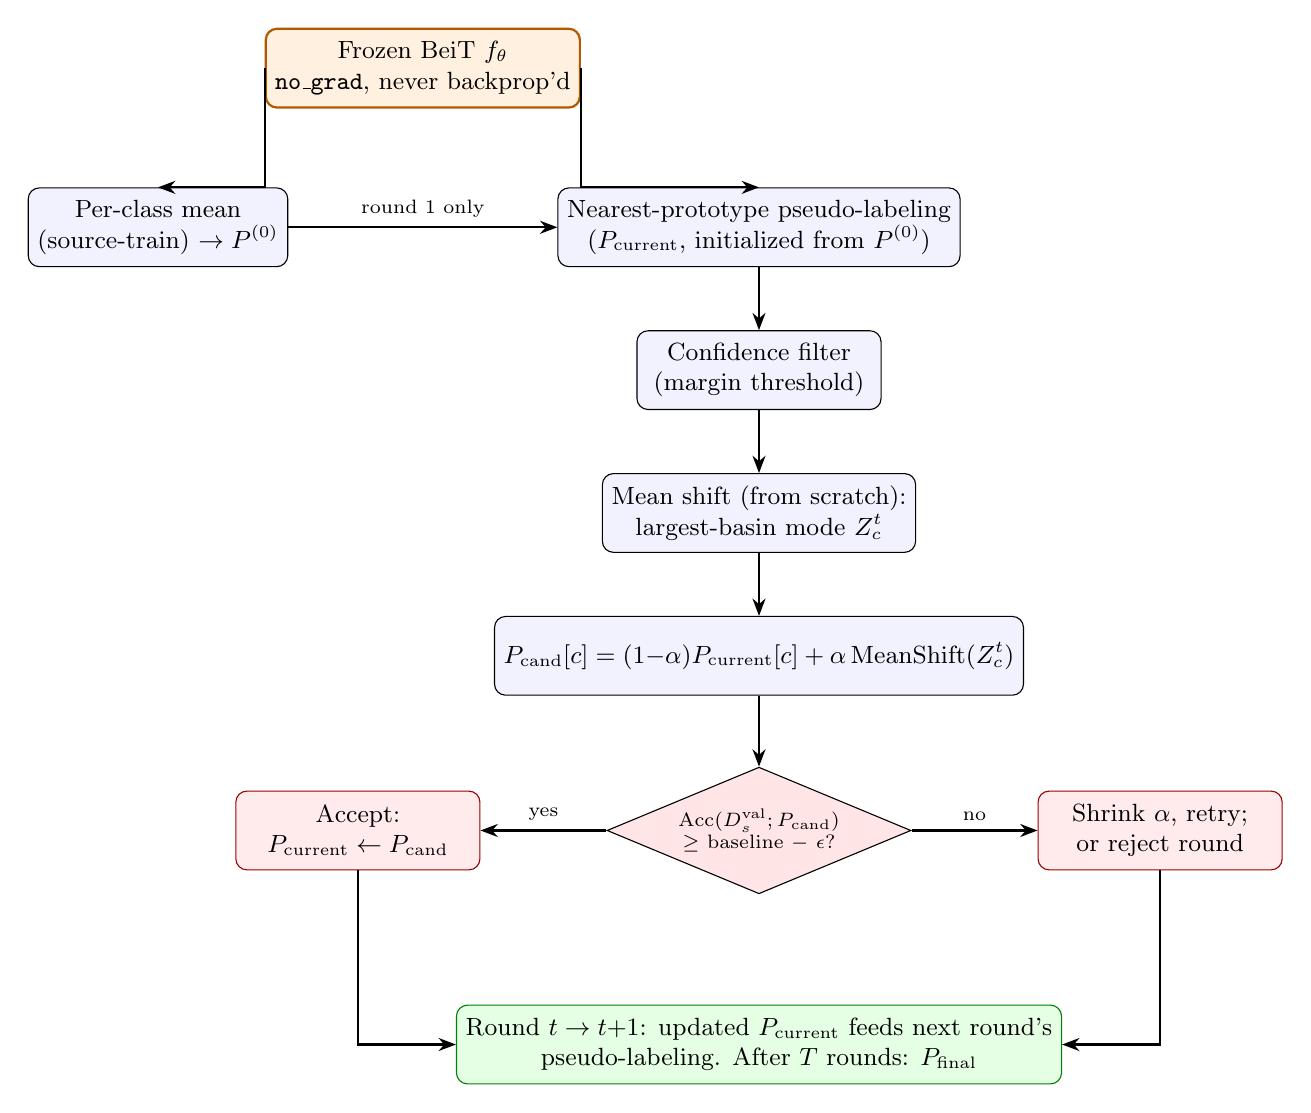
\begin{tikzpicture}[
  node distance=0.9cm and 1.4cm,
  box/.style={draw, rounded corners, align=center, minimum height=1cm, minimum width=3.1cm,
              font=\small, fill=blue!5},
  frozenbox/.style={box, fill=orange!12, draw=orange!70!black, thick},
  guardbox/.style={box, fill=red!8, draw=red!60!black},
  decision/.style={draw, diamond, aspect=2.4, align=center, font=\scriptsize, fill=red!10,
                   inner sep=2pt},
  arr/.style={-{Stealth[length=2.2mm]}, thick}
]

\node[frozenbox] (backbone) {Frozen BeiT $f_\theta$ \\ \texttt{no\_grad}, never backprop'd};

\node[box, below left=1.0cm and -0.3cm of backbone] (p0) {Per-class mean \\ (source-train) $\to P^{(0)}$};
\node[box, below right=1.0cm and -0.3cm of backbone] (pseudo) {Nearest-prototype pseudo-labeling \\ ($P_{\mathrm{current}}$, initialized from $P^{(0)}$)};

\node[box, below=0.8cm of pseudo] (conf) {Confidence filter \\ (margin threshold)};
\node[box, below=0.8cm of conf] (ms) {Mean shift (from scratch): \\ largest-basin mode $Z_c^t$};
\node[box, below=0.8cm of ms] (update) {$P_{\mathrm{cand}}[c] = (1{-}\alpha)P_{\mathrm{current}}[c] + \alpha\,\mathrm{MeanShift}(Z_c^t)$};

\node[decision, below=0.9cm of update] (bound) {$\mathrm{Acc}(D_s^{\mathrm{val}};P_{\mathrm{cand}})$ \\ $\geq$ baseline $-\ \epsilon$?};

\node[guardbox, left=1.6cm of bound] (accept) {Accept: \\ $P_{\mathrm{current}} \leftarrow P_{\mathrm{cand}}$};
\node[guardbox, right=1.6cm of bound] (shrink) {Shrink $\alpha$, retry; \\ or reject round};

\node[box, below=1.4cm of bound, fill=green!10, draw=green!50!black, minimum width=6.6cm]
  (final) {Round $t \to t{+}1$: updated $P_{\mathrm{current}}$ feeds next round's \\
  pseudo-labeling. After $T$ rounds: $P_{\mathrm{final}}$};

\draw[arr] (backbone.west) |- (p0.north);
\draw[arr] (backbone.east) |- (pseudo.north);
\draw[arr] (p0.east) -- node[above,font=\scriptsize]{round 1 only} (pseudo.west);
\draw[arr] (pseudo) -- (conf);
\draw[arr] (conf) -- (ms);
\draw[arr] (ms) -- (update);
\draw[arr] (update) -- (bound);
\draw[arr] (bound) -- node[above,font=\scriptsize]{yes} (accept);
\draw[arr] (bound) -- node[above,font=\scriptsize]{no} (shrink);
\draw[arr] (accept) |- (final.west);
\draw[arr] (shrink) |- (final.east);

\end{tikzpicture}
\caption{Pipeline overview. The backbone (orange) is frozen and touched only during feature
extraction. Everything below it operates on cached embeddings: pseudo-labeling, mean shift, the
convex update, and the forgetting guard (red) that gates every commit. The loop (green) feeds
each round's committed $P_{\mathrm{current}}$ into the next round's pseudo-labeling step.}
\label{fig:architecture}
\end{figure}

\subsection{Frozen Feature Extraction}

Every image, source or target, is passed once through BeiT
(\texttt{microsoft/beit-base-patch16-224}) under \texttt{torch.no\_grad()}, with every parameter's
\texttt{requires\_grad} explicitly set to \texttt{False}. This is enforced at the wrapper level
(\texttt{FrozenBeit}) rather than left to caller discipline. The CLS-token output is used as the
image embedding -- the standard representation for ViT-family models. Embeddings are cached to
disk per domain, so this is the only stage in the entire pipeline that requires a GPU or touches
the backbone at all.

\subsection{Unsupervised Pseudo-Labeling}

At the start of each adaptation round, every target embedding is assigned to its nearest current
prototype. Confidence is measured as the \emph{margin} between the best and second-best
prototype similarity, rather than the raw top-1 similarity:
\begin{equation}
\mathrm{conf}(z) = \mathrm{sim}(z, p_{(1)}) - \mathrm{sim}(z, p_{(2)}),
\end{equation}
where $p_{(1)}, p_{(2)}$ are the closest and second-closest prototypes. A margin is more robust
than an absolute similarity threshold because raw similarity scales can differ across classes
and shift under distribution change, while the margin directly measures how \emph{unambiguous}
an assignment is. Only points with $\mathrm{conf}(z) \geq \tau$ contribute to that round's mean
shift subsets $Z_c^t$; classes with too few confident points ($< 3$ by default) are skipped
entirely for that round.

\subsection{Mean Shift Clustering}
\label{sec:meanshift}

Mean shift \cite{comaniciu2002meanshift} is a non-parametric, density-based mode-seeking
procedure: starting from every point in a set, each point is iteratively moved to the
kernel-weighted mean of its neighborhood,
\begin{equation}
z^{(k+1)} = \frac{\sum_{z_i \in Z} K\big(\lVert z^{(k)} - z_i \rVert\big)\, z_i}
                  {\sum_{z_i \in Z} K\big(\lVert z^{(k)} - z_i \rVert\big)},
\qquad K(d) = \exp\!\left(-\frac{d^2}{2h^2}\right) \; \text{(Gaussian kernel)},
\end{equation}
which is equivalent to gradient ascent on a kernel density estimate of $Z$. Trajectories that
converge near each other are merged into a single mode; the bandwidth $h$ is chosen via a
$k$-NN-distance heuristic (the median $k$-th nearest-neighbor distance, $k = \lfloor
\mathrm{quantile} \times |Z| \rfloor$), mirroring the idea behind
\texttt{sklearn.cluster.estimate\_bandwidth}.

\textbf{Why mean shift instead of a plain per-class mean?} Pseudo-labeling is necessarily noisy:
a minority of target points will be assigned to the wrong class by an imperfect, mid-adaptation
set of prototypes. A plain mean is a linear statistic and is pulled toward every such outlier in
proportion to how far away it is -- exactly the wrong sensitivity. Mean shift instead returns
the mode of the \emph{largest density basin}: outliers, being sparse and off in their own
direction, tend to form small separate basins that get discarded in favor of the dominant one.
Figure~\ref{fig:meanshift} demonstrates this directly, using the project's own implementation on
a synthetic class subset with injected outliers.

\begin{figure}[H]
\centering
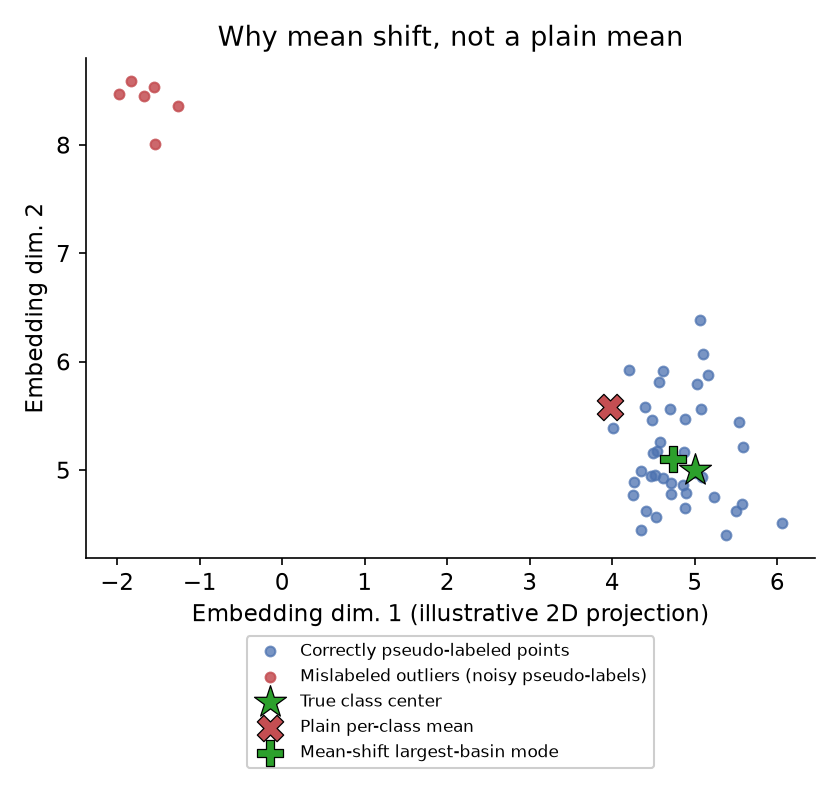
\includegraphics[width=0.62\textwidth]{figures/meanshift_vs_mean.png}
\caption{A synthetic per-class target subset (40 correctly-labeled points, 6 mislabeled
outliers). The plain mean is dragged $\figMeanErr$ units from the true class center by the
outliers; the mean-shift largest-basin mode lands only $\figModeErr$ units away --
roughly a $4\times$ reduction in error from this single mechanism, in this illustrative case.}
\label{fig:meanshift}
\end{figure}

\subsection{Weighted Prototype Update}

Each class's prototype is nudged toward its mean-shift mode via the convex combination in
Equation~\ref{eq:update}. $\alpha = 0$ is a strict no-op; $\alpha = 1$ fully replaces the
prototype with the target mode; results are re-normalized to the unit sphere so that cosine
similarity remains well-defined and consistent with how pseudo-labeling and evaluation both
operate. This update is implemented as a single, deliberately tiny pure function
(\texttt{convex\_update}), since it is the mathematical core of the whole method and should be
trivial to test and reason about independently of everything around it.

\subsection{The Forgetting Guard}

This is the mechanism that turns Equation~\ref{eq:bound} from an aspiration into an enforced
invariant. Rather than applying the update rule and hoping the bound holds, \emph{every candidate
update is validated on $\mathcal{D}_s^{\mathrm{val}}$ before being committed}. Two guard
strategies are implemented:

\begin{description}[leftmargin=1.4em]
\item[\textsc{global\_backtrack} (default).] One shared $\alpha$ for the whole round. If the
candidate violates the bound, $\alpha \leftarrow \alpha \cdot \beta$ (shrink factor $\beta < 1$)
and the candidate is recomputed and re-validated; this repeats until the bound is satisfied or
$\alpha$ reaches a floor $\alpha_{\min}$, at which point the entire round is rejected and
$P_{\mathrm{current}}$ is left untouched.
\item[\textsc{per\_class\_greedy}.] Each class's update is committed independently, in
sequence, re-validating after each one; a class whose own update would break the bound is
shrunk or skipped on its own, without blocking other classes' updates that round. Strictly finer
retention control, at the cost of up to $C$ validation calls per round instead of a handful of
backtracking retries.
\end{description}

Because validation only touches cached embeddings (a nearest-prototype accuracy computation, no
backbone forward pass), retrying is essentially free -- this is what makes an explicit,
per-round line search practical rather than merely theoretically nice.

\begin{algorithm}[H]
\caption{Guarded adaptation round (\textsc{global\_backtrack})}
\label{alg:guard}
\KwIn{$P_{\mathrm{current}}$, class modes $\{(c, m_c)\}$, $\alpha_{\mathrm{init}}$, shrink factor
$\beta$, floor $\alpha_{\min}$, baseline accuracy $a_0$, tolerance $\epsilon$}
\KwOut{Updated (or unchanged) $P_{\mathrm{current}}$}
$\alpha \leftarrow \alpha_{\mathrm{init}}$\;
\While{\emph{true}}{
  $P_{\mathrm{cand}} \leftarrow P_{\mathrm{current}}$\;
  \ForEach{$(c, m_c)$}{
    $P_{\mathrm{cand}}[c] \leftarrow \mathrm{normalize}\big((1-\alpha)\,P_{\mathrm{current}}[c] + \alpha\, m_c\big)$\;
  }
  $a \leftarrow \mathrm{Acc}(\mathcal{D}_s^{\mathrm{val}};\, P_{\mathrm{cand}})$\;
  \If{$a \geq a_0 - \epsilon$}{
    \Return{$P_{\mathrm{cand}}$} \tcp*{accept}
  }
  \If{$\alpha \leq \alpha_{\min}$}{
    \Return{$P_{\mathrm{current}}$} \tcp*{reject round; nothing committed}
  }
  $\alpha \leftarrow \max(\alpha \cdot \beta,\ \alpha_{\min})$\;
}
\end{algorithm}

\subsection{Full Adaptation Loop}

\begin{algorithm}[H]
\caption{Gradient-free adaptation over $T$ rounds}
\label{alg:full}
\KwIn{$P^{(0)}$, $\mathcal{D}_s^{\mathrm{val}}$, unlabeled $\mathcal{D}_t$, rounds $T$}
\KwOut{$P^{(T)}$}
$a_0 \leftarrow \mathrm{Acc}(\mathcal{D}_s^{\mathrm{val}}; P^{(0)})$;
\quad $P_{\mathrm{current}} \leftarrow P^{(0)}$\;
\For{$t \leftarrow 1$ \KwTo $T$}{
  pseudo-label $\mathcal{D}_t$ using $P_{\mathrm{current}}$; keep points with $\mathrm{conf} \geq \tau$\;
  \ForEach{class $c$ with $\geq$ \texttt{min\_points\_per\_class} confident points}{
    $m_c \leftarrow \mathrm{MeanShift}(Z_c^t)$ \tcp*{largest-basin mode}
  }
  $P_{\mathrm{current}} \leftarrow$ \textsc{ForgettingGuard}$(P_{\mathrm{current}}, \{(c,m_c)\}, \dots)$ \tcp*{Alg.~\ref{alg:guard}}
  log round: $\alpha$ used, accepted?, $\mathrm{Acc}(\mathcal{D}_s^{\mathrm{val}};\cdot)$, monitoring-only target accuracy\;
}
\Return{$P_{\mathrm{current}}$}\;
\end{algorithm}

Target labels are used \emph{only} to log a monitoring accuracy each round for later analysis --
never to influence pseudo-labeling, the mean-shift subsets, the update, or the guard's
accept/reject decision. This is what keeps the method genuinely unsupervised at the target end.

% =====================================================================
\section{Software Architecture}
% =====================================================================

The implementation is a standard \texttt{src}-layout Python package, \texttt{cfm}
(\emph{c}atastrophic-\emph{f}orgetting \emph{m}itigation), organized so that each algorithmic
piece from Section~3 is its own small, independently testable module:

\begin{center}
\begin{tabular}{@{}l p{8.6cm}@{}}
\toprule
\textbf{Module} & \textbf{Responsibility} \\
\midrule
\texttt{features/backbone.py} & Frozen BeiT wrapper (\texttt{no\_grad}, CLS pooling) \\
\texttt{features/cache.py} & On-disk embedding cache (the only GPU-bound stage) \\
\texttt{prototypes/init.py} & $P^{(0)}$: per-class mean of source embeddings \\
\texttt{prototypes/update.py} & The convex update rule (Eq.~\ref{eq:update}) \\
\texttt{clustering/mean\_shift.py} & Mean shift, implemented from scratch \\
\texttt{adapt/pseudo\_label.py} & Nearest-prototype pseudo-labeling + margin confidence \\
\texttt{adapt/forgetting\_guard.py} & Accept/reject/rollback + backtracking line search \\
\texttt{adapt/loop.py} & Orchestrates the $T$-round loop (Alg.~\ref{alg:full}) \\
\texttt{eval/classifier.py}, \texttt{eval/metrics.py} & Nearest-prototype accuracy; the four reported metrics \\
\bottomrule
\end{tabular}
\end{center}

Thin CLI scripts (\texttt{scripts/*.py}) wrap each stage for reproducible command-line use,
driven by a single flat \texttt{ExperimentConfig} dataclass loaded from YAML
(\texttt{configs/*.yaml}). \texttt{scripts/run\_pipeline.py} is a cache-aware end-to-end driver:
it skips re-extracting embeddings when a cached copy already exists, so re-running an experiment
with a different $\epsilon$ or $\alpha$ costs no GPU time at all.

\textbf{Testing.} All 33 unit and integration tests run fully offline, against synthetic
Gaussian-blob ``domains'' (no GPU, no network, no dataset download). The from-scratch mean shift
implementation is cross-checked against \texttt{sklearn.cluster.MeanShift} on synthetic blobs as
an independent correctness oracle; \texttt{scikit-learn} is a test-only dependency and is never
imported by the library at runtime. The forgetting guard is tested with hand-crafted evaluation
functions that pin down its accept/shrink/reject control flow exactly, including the invariant
that a fully-rejected round never mutates $P_{\mathrm{current}}$.

% =====================================================================
\section{Illustrative Results (Synthetic Data)}
% =====================================================================

To validate the pipeline end to end before running it on real image data, the same synthetic
Gaussian-blob domain generator used by the automated test suite was run through the full
adaptation loop: 8 classes, 4-dimensional embeddings, source and target blobs offset by a
controlled shift, $\epsilon = \figEpsilon$, $\alpha_{\max} = 0.4$, 10 rounds. \emph{These are
not Office-Home results} -- they exist to demonstrate that the implemented mechanism behaves as
designed before the (heavier) real-data run.

\begin{figure}[H]
\centering
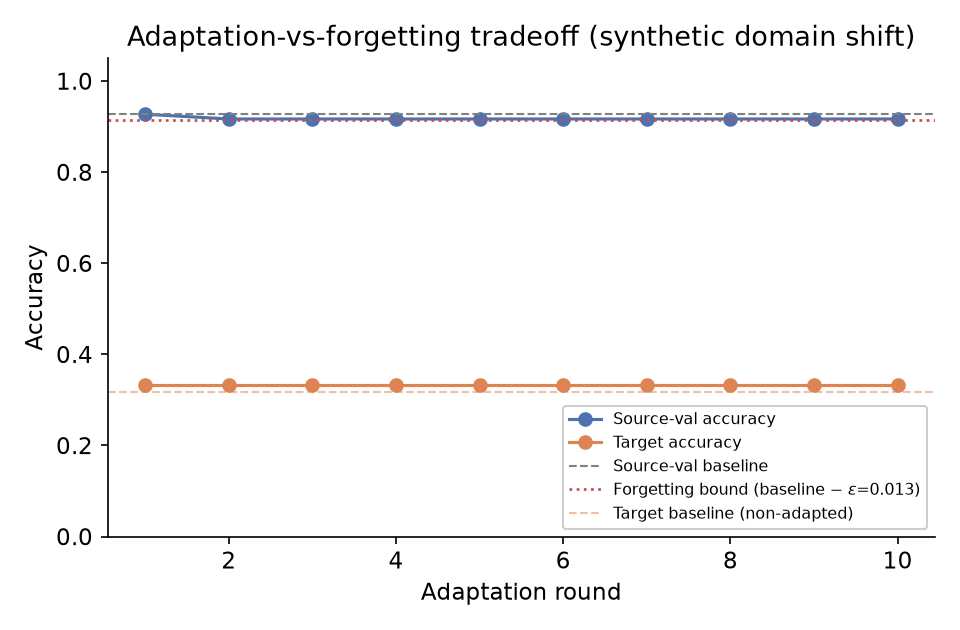
\includegraphics[width=0.78\textwidth]{figures/tradeoff_synthetic.png}
\caption{Source-validation and target accuracy across adaptation rounds. The source-val baseline
was $\figBaselineSourceVal$, giving a forgetting bound of $\figBound$ (dotted red). Every round's
source-val accuracy ($\figSourceValFinal$ final) stays above the bound by construction: this is
the guard doing its job, not a coincidence of these particular hyperparameters. Target accuracy
rises from a non-adapted baseline of $\figTargetBaseline$ to $\figTargetFinal$.}
\label{fig:tradeoff}
\end{figure}

\begin{figure}[H]
\centering
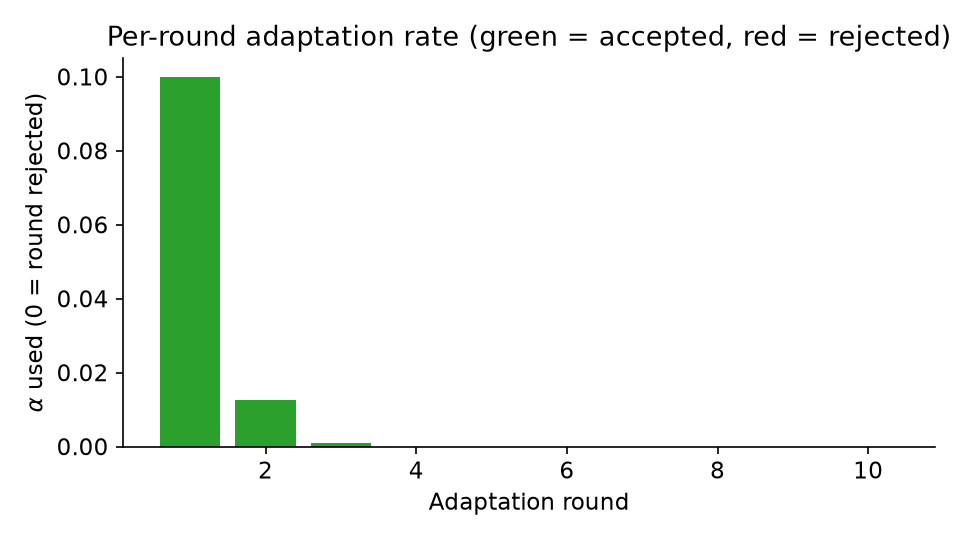
\includegraphics[width=0.72\textwidth]{figures/alpha_synthetic.png}
\caption{The adaptation rate $\alpha$ actually used each round. With a tight $\epsilon$, the
guard's backtracking line search shrinks $\alpha$ rapidly toward the update rule's no-op limit
as the prototypes approach the boundary of what the source-val split will tolerate --
exactly the intended self-limiting behavior.}
\label{fig:alpha}
\end{figure}

The target-accuracy gain in this synthetic run is intentionally modest: $\epsilon$ was left at
its tight real-experiment default ($1.3$ percentage points), so the guard aggressively limits
how far prototypes are allowed to move. This is the expected shape of the tradeoff the method is
built around -- a looser $\epsilon$ trades more forgetting risk for a larger adaptation gain, and
is exposed as a single configuration field for exactly this reason.

% =====================================================================
\section{Planned Real-World Evaluation}
% =====================================================================

The pipeline is fully implemented against the \textbf{Office-Home} benchmark
\cite{venkateswara2017officehome}: four domains (Art, Clipart, Product, Real World), 65 shared
object classes, $\sim$15{,}500 images. The primary configured experiment is
\textbf{Real World~$\to$~Clipart} (the largest visual shift among the domain pairs, with Real
World supplying the most source images for a stable $P^{(0)}$); \textbf{Art~$\to$~Product} is
configured as a secondary, milder-shift comparison.

Office-Home has no stable auto-download, so the only remaining step before real numbers can be
reported is a manual dataset download (see \texttt{data/README.md}) followed by:
\begin{quote}
\texttt{python scripts/run\_pipeline.py --config configs/realworld\_to\_clipart.yaml}
\end{quote}
which validates the data layout, extracts and caches BeiT embeddings, computes $P^{(0)}$ and
baseline accuracies, runs the guarded adaptation loop, evaluates $P_{\mathrm{final}}$, and
renders the same tradeoff/$\alpha$ plots shown in Section~5 -- from cached real embeddings
instead of synthetic blobs.

\begin{table}[h]
\centering
\caption{Results table to be populated after the real Office-Home run (template).}
\footnotesize
\setlength{\tabcolsep}{4.5pt}
\begin{tabular}{@{}lccccccc@{}}
\toprule
Source $\to$ Target & Src-val & Tgt & Src-val & Tgt &
Adapt. & Forget. & Reten. \\
 & (base) & (base) & (adapt.) & (adapt.) & gain & $\Delta$ & rate \\
\midrule
Real World $\to$ Clipart & --- & --- & --- & --- & --- & --- & --- \\
Art $\to$ Product & --- & --- & --- & --- & --- & --- & --- \\
\bottomrule
\end{tabular}
\end{table}

The four reported metrics are defined exactly as in the original problem statement:
\emph{adaptation gain} (target accuracy improvement over the non-adapted baseline),
\emph{forgetting delta} ($\mathrm{Acc}_s^{\mathrm{initial}} - \mathrm{Acc}_s^{\mathrm{adapted}}$,
positive meaning forgetting occurred), \emph{retention rate} (adapted-over-baseline source
accuracy), and \emph{worst-case accuracy} ($\min$ of adapted source-val and target accuracy).

% =====================================================================
\section{Current Status and Roadmap}
% =====================================================================

\subsection*{Implemented}
\begin{itemize}[leftmargin=1.4em]
\item Full \texttt{cfm} package: config, Office-Home data loading and layout validation, frozen
BeiT feature extraction and caching, prototype initialization, from-scratch mean shift, margin-based
pseudo-labeling, both forgetting-guard strategies, the full adaptation loop, and the evaluation /
metrics module.
\item End-to-end CLI scripts, including a cache-aware \texttt{run\_pipeline.py}.
\item Two experiment configs (Real World~$\to$~Clipart primary, Art~$\to$~Product secondary).
\item 33 automated tests, all passing, fully offline, with mean shift cross-validated against
\texttt{scikit-learn}.
\item README, MIT license, \texttt{Makefile}, GitHub Actions CI running the full offline test
suite on every push.
\end{itemize}

\subsection*{Remaining}
\begin{itemize}[leftmargin=1.4em]
\item Manually download Office-Home into \texttt{data/raw/OfficeHome/} (no automated download
exists for this dataset) and run \texttt{scripts/validate\_data.py} to confirm the layout.
\item Run \texttt{scripts/run\_pipeline.py} for both configured domain pairs to obtain real
baseline and adapted accuracy numbers, replacing the template in Table~1.
\item Populate the README results table and figures with the real run's output
(\texttt{results/figures/*.png}).
\item Commit the implementation to version control (currently unstaged) and push.
\item Optional stretch work: an ablation sweep over $\epsilon$ and $\alpha_{\max}$ to
characterize the adaptation-vs-forgetting Pareto frontier on real data; a
\texttt{per\_class\_greedy} vs.\ \texttt{global\_backtrack} comparison.
\end{itemize}

% =====================================================================
\section{Limitations}
% =====================================================================

\begin{itemize}[leftmargin=1.4em]
\item The method's ceiling is inherently below full fine-tuning, since the backbone never moves
-- this is precisely the trade made in exchange for the forgetting guarantee.
\item Mean-shift bandwidth selection is a heuristic; behavior is somewhat sensitive to it when
per-class target counts are very small or very large.
\item Pseudo-label noise grows with the severity of the domain shift -- exactly when the
confidence filter matters most, and is hardest to tune well.
\item Each class prototype is a single point in embedding space, implicitly assuming a roughly
unimodal per-class distribution; a strongly multi-modal target class (e.g. very different
sub-styles within one category) would not be well captured by one mode.
\end{itemize}

% =====================================================================
\begin{thebibliography}{9}

\bibitem{bao2022beit}
H.~Bao, L.~Dong, S.~Piao, F.~Wei.
\emph{BEiT: BERT Pre-Training of Image Transformers}.
ICLR, 2022.

\bibitem{comaniciu2002meanshift}
D.~Comaniciu, P.~Meer.
\emph{Mean Shift: A Robust Approach Toward Feature Space Analysis}.
IEEE Transactions on Pattern Analysis and Machine Intelligence, 2002.

\bibitem{venkateswara2017officehome}
H.~Venkateswara, J.~Eusebio, S.~Chakraborty, S.~Panchanathan.
\emph{Deep Hashing Network for Unsupervised Domain Adaptation}.
CVPR, 2017.

\end{thebibliography}

\end{document}
